%\ctparttext{\color{black}\begin{center}
%		Esta es una descripción de la parte de informática.
%\end{center}}

%\part{Parte de informática}
\chapter{Instalación de las máquinas virtuales}

Comenzamos descargando Ubuntu Server, en su versión 20.04 LTS.

Abrimos VirtualBox y creamos dos máquinas virtuales, m1-anabuenrua y m2-anabuenrua, asignando a cada una 1GB de RAM y 10GB de disco duro dinámico.

Añadimos en ambas Ubuntu Server pulsando en añadir unidad óptica en la configuración de cada máquina virtual.

Así, las máquinas virtuales ya están listas para arrancar. Se va a explicar cómo se realiza la configuración de una de ellas, la otra se haría de manera análoga.

Procedemos a lanzar la máquina m1-anabuenrua y empezamos la configuración:

Seleccionamos el idioma español, y en la siguiente pantalla en "detectar teclado", de forma que tras pulsar las teclas que nos pide, nos detecta la variante española del teclado.

En los siguientes pasos dejamos la configuración por defecto.

Introduzco mi nombre y mi usuario de la ugr con contraseña \verb|Swap1234| como se muestra en \eqref{instalacion_nombre}.

\begin{figure}
\begin{center}
\caption{Introduzco mi nombre y usuario de la ugr, con contraseña "Swap1234"  durante la instalación de la máquina virtual m1-anabuenrua}
\label{instalacion_nombre}
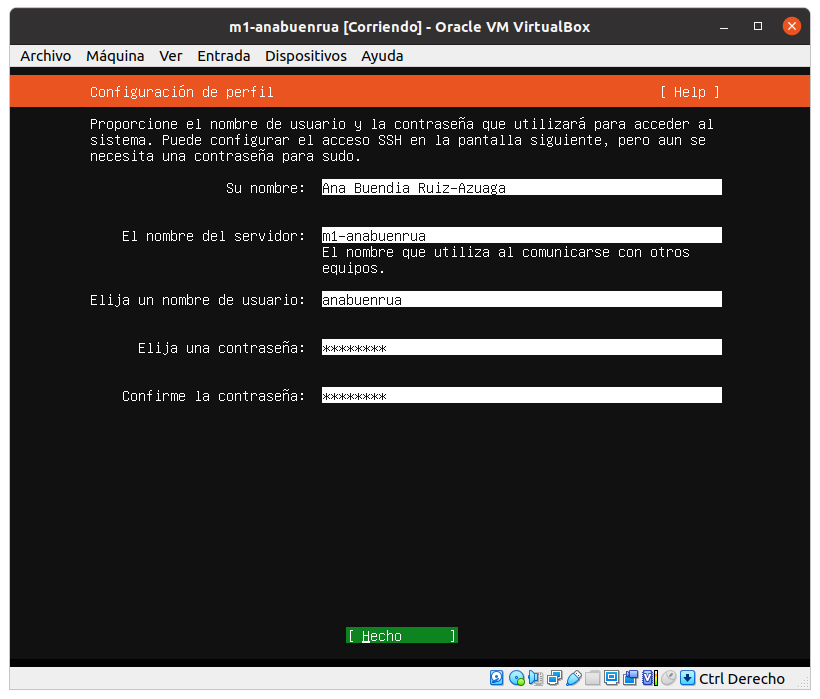
\includegraphics[scale=0.5]{so_config_11}
\end{center}
\end{figure}

Tras esto, seguimos con la instalación por defecto, indicando que instale ssh durante la instalación.

Una vez terminada la instalación reiniciamos la máquina y comprobamos que en efecto funciona correctamente.

Finalmente activamos la cuenta de root mediante la ejecución de \verb|sudo passwd root|.

Repetimos el mismo procedimiento con la otra máquina virtual.

\chapter{Configuración de la red}

\section{Configuración básica}

Para disponer de conexión a internet y poder conectar las máquinas entre sí y con el anfitrión vamos a añadir un adaptador de red en modo NAT y otro adaptador de red solo-anfitrión.

Comenzamos con la red NAT, que ya venía por defecto, como se ve en \eqref{red_NAT}:

\begin{figure}
\begin{center}
\caption{Configuración de red NAT}
\label{red_NAT}
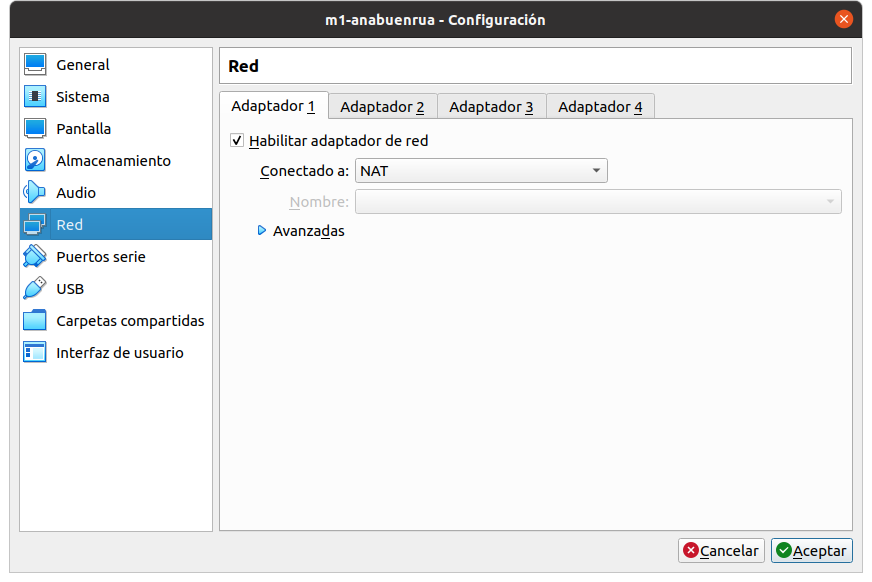
\includegraphics[scale=0.5]{red_1}
\end{center}
\end{figure}

A continuación, como no tengo configurada la red solo-anfitrión en mi VirtualBox voy a crear una, en \verb|archivo->Administrador de red anfitrión| añado la red \verb|vboxnet0| como se muestra en \eqref{red_crear_vboxnet0}

\begin{figure}
\begin{center}
\caption{Creación de la red solo-anfitrión vboxnet0}
\label{red_crear_vboxnet0}
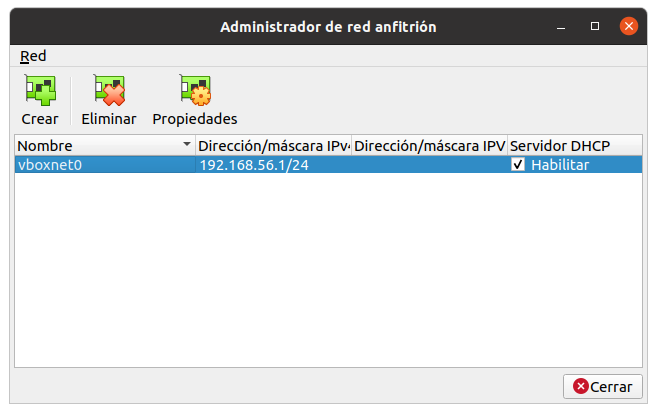
\includegraphics[scale=0.5]{red_3}
\end{center}
\end{figure}

Una vez creada, configuramos en nuestra máquina virtual la red solo-anfitrión, como puede verse en \eqref{red_hostonly}:

\begin{figure}
\begin{center}
\caption{Configuración de red solo-anfitrión}
\label{red_hostonly}
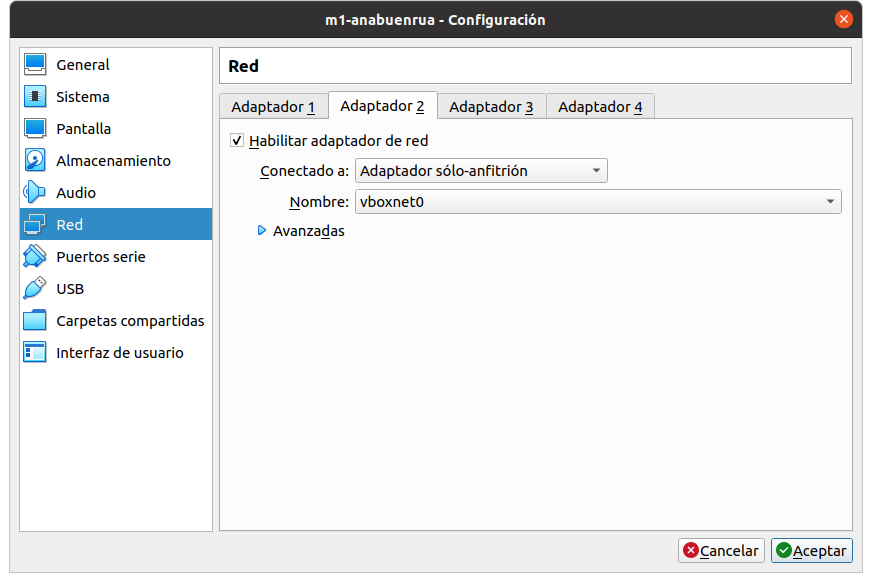
\includegraphics[scale=0.5]{red_2}
\end{center}
\end{figure}

Lanzamos la máquina virtual para completar la configuración de la red editando el fichero \verb|/etc/netplan/00-installer-config.yaml|, dejándolo como se muestra en \eqref{red_archivo}:

\begin{figure}
\begin{center}
\caption{Archivo /etc/netplan/00-installer-config.yaml de configuración de red}
\label{red_archivo}
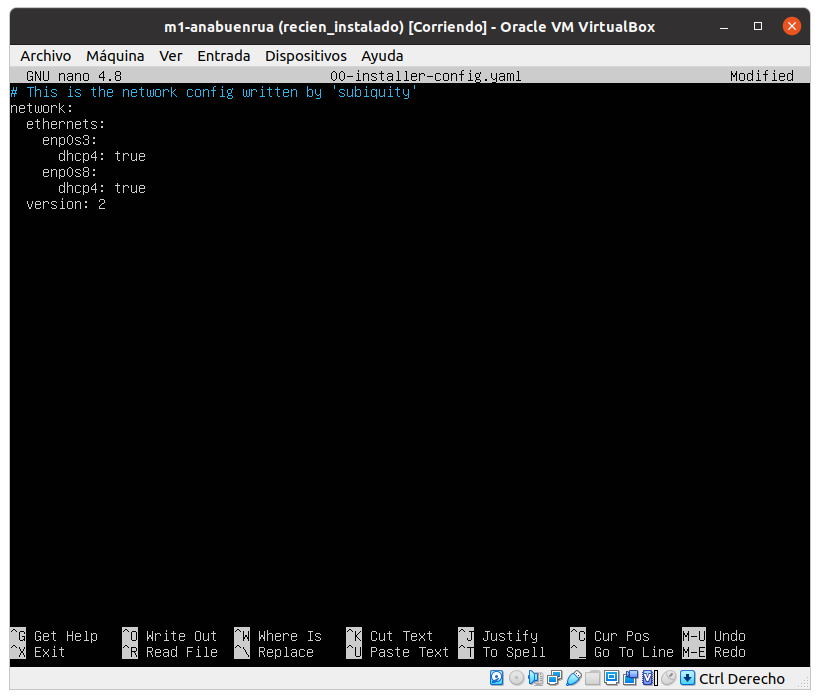
\includegraphics[scale=0.5]{red_4}
\end{center}
\end{figure}

Finalmente ejecutamos el comando \verb|sudo netplan apply| para hacer efectivos los cambios.

Comprobamos con el comando \verb|ip address show| que la configuración se ha realizado correctamente, mostrando \verb|enp0s8| y su dirección ip, obteniendo la salida de \eqref{red_ip}.

\begin{figure}
\begin{center}
\caption{Resultado de la ejecución del comando ip address show en la máquina m1-anabuenrua}
\label{red_ip}
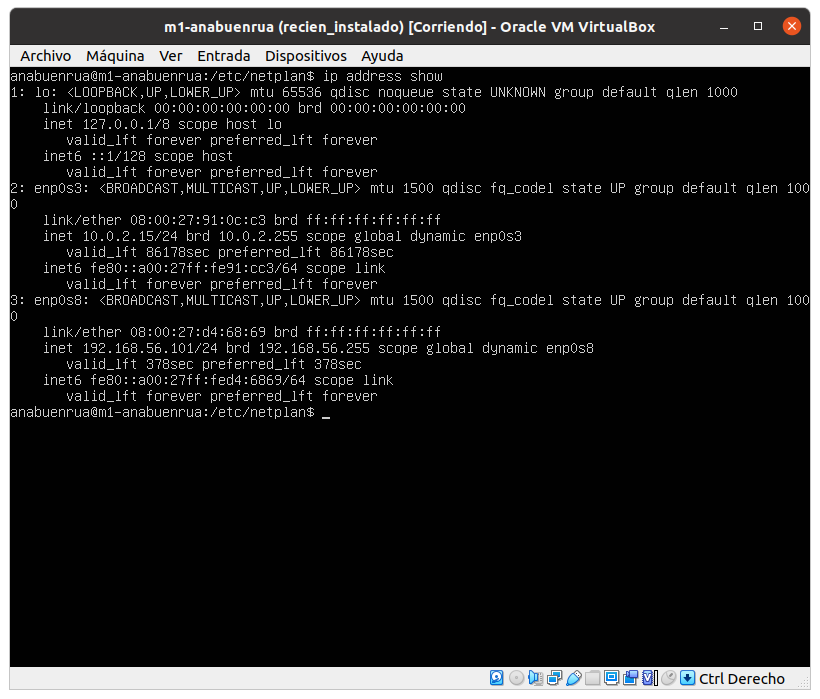
\includegraphics[scale=0.5]{red_6}
\end{center}
\end{figure}


Finalmente comprobamos mediante ping que podemos conectarnos entre las máquinas. La dirección ip de la máquina m1 es \verb|192.168.56.101|, mientras la de la máquina m2 es \verb|192.168.56.102|.

\section{Configuración avanzada}

Para realizar la configuración avanzada de la red, de nuevo se hará modificando el fichero \verb|/etc/netplan/00-installer-config.yaml|. Vamos a asignar las direcciones IPs , aunque no vamos a cambiarlas. A la máquina m1 se le asignará \verb|192.168.56.101| y a m2 \verb|192.168.56.102|, y en ambas se usará la máscara de red \verb|255.255.255.0|, por lo que añadimos un \verb|/24| al final de las ips como se muestra en \eqref{red_archivo2}.

\begin{figure}[h!]
\begin{center}
\caption{Archivo /etc/netplan/00-installer-config.yaml de configuración de red}
\label{red_archivo2}
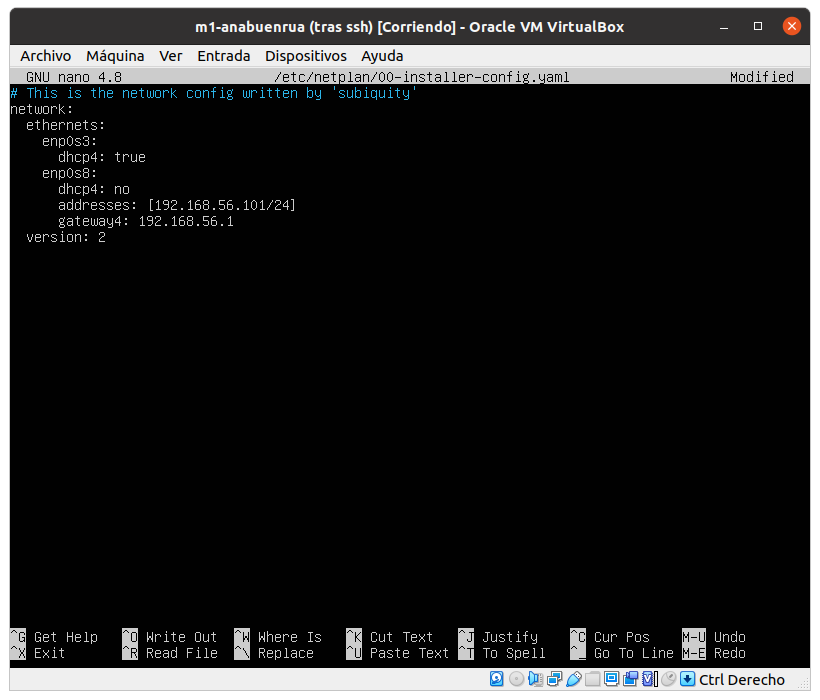
\includegraphics[scale=0.5]{red_avanzada_1}
\end{center}
\end{figure}

Finalmente hacemos efectivos los cambios con \verb|sudo netplan apply|..

Comprobamos con el comando \verb|ip address show| que la configuración se ha realizado correctamente de nuevo.

Para asegurarnos de que todo está bien configurado, realizamos ping de m1 a m2 y después de m2 a m1, confirmando que las máquinas pueden conectarse entre sí. Por ejemplo, la conexión de m1 a m2 puede verse en \eqref{red_ping}.

\begin{figure}[h!]
\begin{center}
\caption{Resultado de la conexión mediante ping de la máquina m1 a m2}
\label{red_ping}
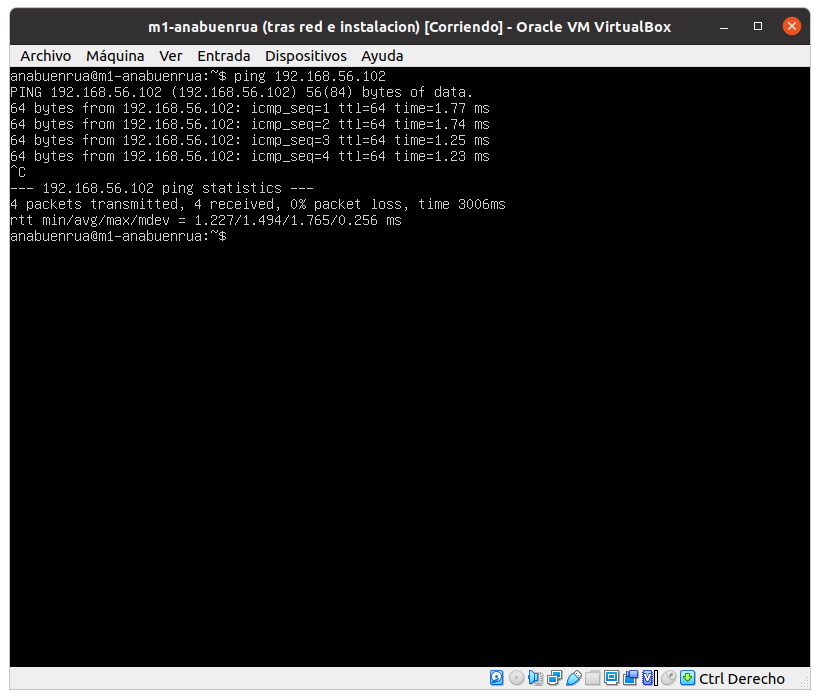
\includegraphics[scale=0.5]{ping_m1m2}
\end{center}
\end{figure}

\chapter{LAMP}

Primero vamos a instalar LAMP, para ello ejecutamos el comando:

\begin{verbatim}
sudo apt-get install apache2 mysql-server mysql-client
\end{verbatim}

Y comprobamos la versión usando \verb|apache2 -v| y si está en ejecución con 

\verb| sudo service apache2 status|, como se ve en \eqref{LAMP_estado}:

\begin{figure}[h!]
\begin{center}
\caption{Comprobación de la versión y estado de apache}
\label{LAMP_estado}
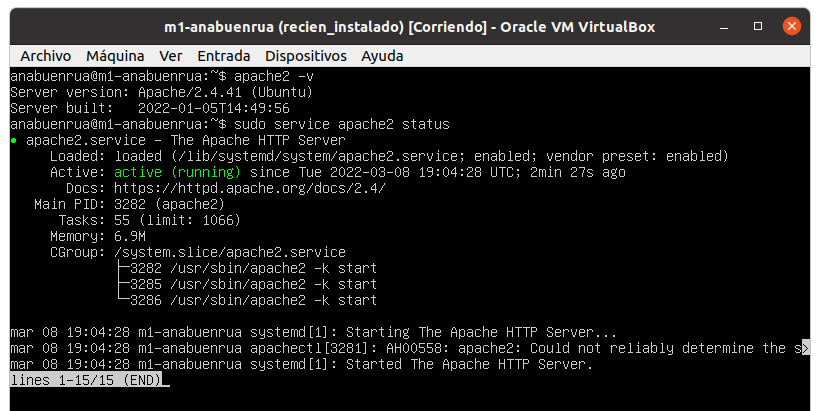
\includegraphics[scale=0.5]{instalar_2}
\end{center}
\end{figure}

Repetimos esta instalación en la otra máquina virtual también.

\section{Fichero swap.html}

Comenzamos creando el archivo \verb|swap.html| en el directorio \verb|/var/www/html/|, con los contenidos:

\begin{verbatim}
<HTML>
<BODY>
Web de ejemplo de anabuenrua para SWAP
Email: anabuenrua@correo.ugr.es
</BODY>
</HTML>
\end{verbatim}

Y comprobamos que se sirve esta página mediante el navegador web de nuestro navegador \eqref{swaphtml} o con curl (lo comprobamos en la sección de curl).

\begin{figure}[h!]
\begin{center}
\caption{Acceso a swap.html desde el navegador.}
\label{swaphtml}
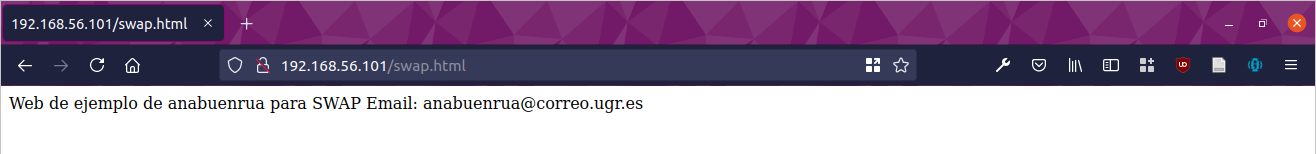
\includegraphics[scale=0.5]{apache_redirect_2}
\end{center}
\end{figure}

Análogamente se puede comprobar cambiando los roles de las máquinas m1 y m2.

\section{Cambiando puertos}

Vamos a cambiar el puerto de escucha al 8081. Para ello comenzamos modificando el fichero \verb|/etc/apache2/ports.conf| añadiendo la línea \verb|Listen 8081|.

A continuación modificamos el archivo \verb|/etc/apache2/sites-enabled/000-default.conf| como se ve en \eqref{apache_puertos}:

\begin{figure}[h!]
\begin{center}
\caption{Fichero de configuracion /etc/apache2/sites-enabled/000-default.conf}
\label{apache_puertos}
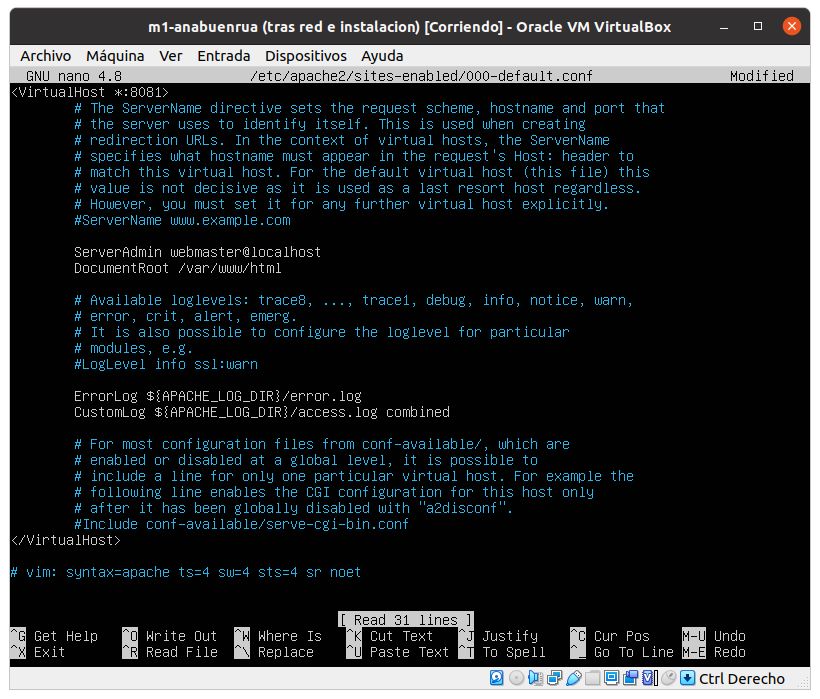
\includegraphics[scale=0.5]{apache_port_2}
\end{center}
\end{figure}

Comprobamos que esté todo bien con \verb|sudo apache2ctl configtest|, que nos devuelve \verb|Syntax OK|, por lo que reiniciamos el servicio apache con \verb|sudo systemctl restart apache2| y comprobamos que el cambio se ha hecho correctamente accediendo a la dirección ip especificando el puerto 8081 como se ve en \eqref{apache_puertos2}.

\begin{figure}[h!]
\begin{center}
\caption{Acceso a apache a través del puerto 8081}
\label{apache_puertos2}
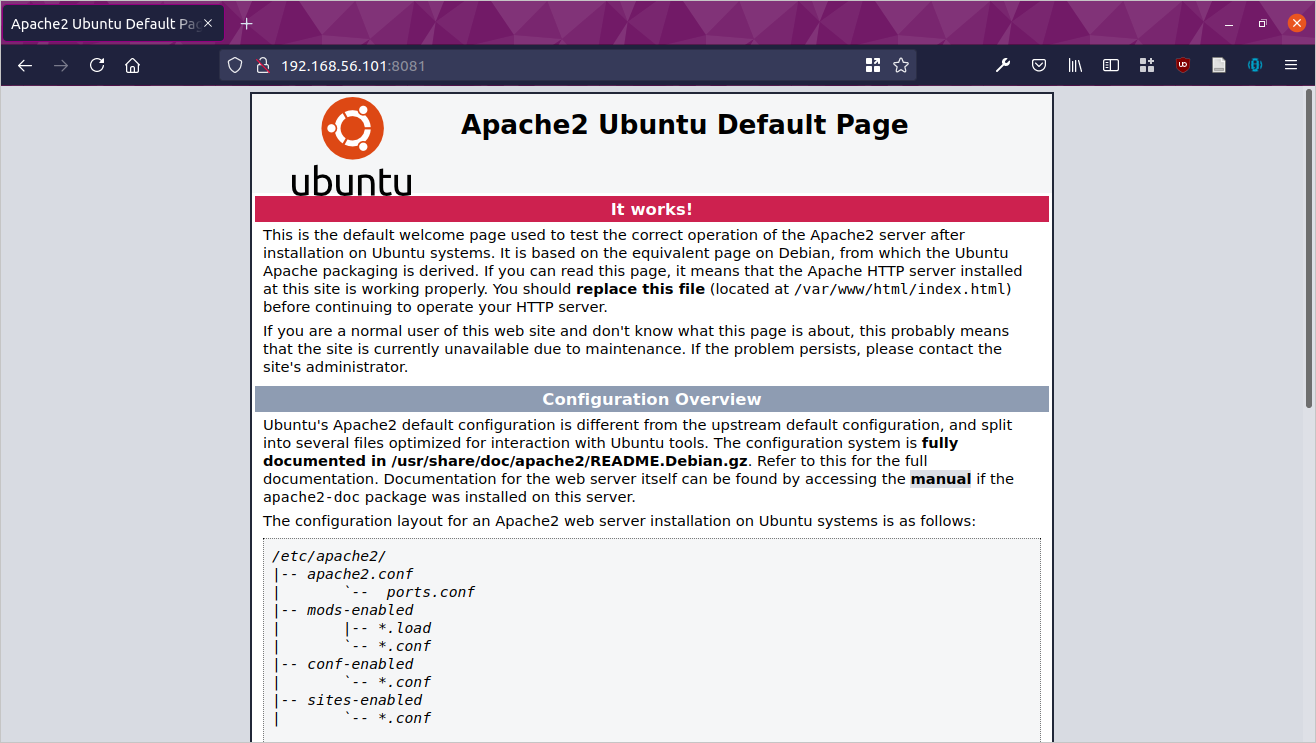
\includegraphics[scale=0.5]{apache_port_3}
\end{center}
\end{figure}

\section{Directorios virtuales}

En \verb|/var/www| creamos la carpeta \verb|prueba/public_html| con el comando 

\verb|sudo mkdir -p prueba/public_html|.

Y en este directorio creamos el archivo \verb|index.html| con el contenido:

\begin{verbatim}
<HTML>
<BODY>
Prueba de directorio virtual
</BODY>
</HTML>
\end{verbatim}

Cambiamos la propiedad de los archivos al usuario de apache con 

\verb|sudo chown -R www-data: /var/www/prueba| y creamos en 

\verb|/etc/apache2/sites-available| el fichero \verb|prueba.conf|, como en \eqref{prueba_conf}

\begin{figure}[h!]
\begin{center}
\caption{Archivo de configuración prueba.conf}
\label{prueba_conf}
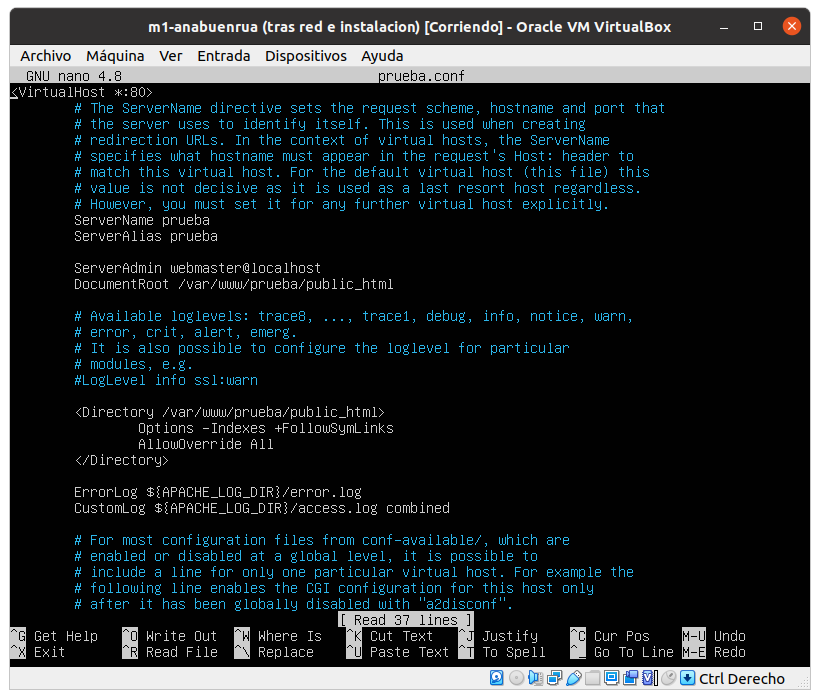
\includegraphics[scale=0.5]{apache_5}
\end{center}
\end{figure}

Finalmente comprobamos que no haya ningún fallo de sintaxis con \verb|sudo apachectl configtest|, y al devolver \verb|syntax OK|  habilitamos el nuevo archivo de host virtual con 

\verb|sudo a2ensite domain1.com| y reiniciamos el servicio de apache con 

\verb|sudo systemctl restart apache2|.

Finalmente comprobamos accediendo desde el navegador que funciona correctamente, como en \eqref{apache_final}

\begin{figure}[h!]
\begin{center}
\caption{Acceso al directorio virtual prueba}
\label{apache_final}
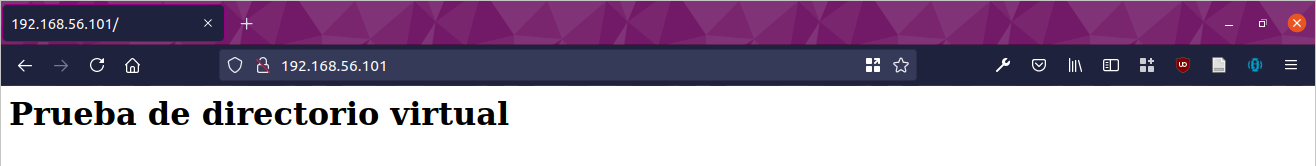
\includegraphics[scale=0.5]{apache_virdir}
\end{center}
\end{figure}

\section{Redirección de puertos}

Como hemos configurado antes, se usa el puerto 8081. Ahora vamos a redireccionar las direcciones al puerto 80 para que las atienda el 8081.

De nuevo en \verb|/etc/apache2/ports.conf| nos aseguramos de que se escuche ambos puertos con \verb|Listen 80| y \verb|Listen 8081|.

Ahora en \verb|/etc/apache2/sites-enabled/000-default.conf| añadimos el bloque \eqref{apache_redireccion}

\begin{figure}[h!]
\begin{center}
\caption{Fichero de configuración /etc/apache2/sites-enabled/000-default.conf}
\label{apache_redireccion}
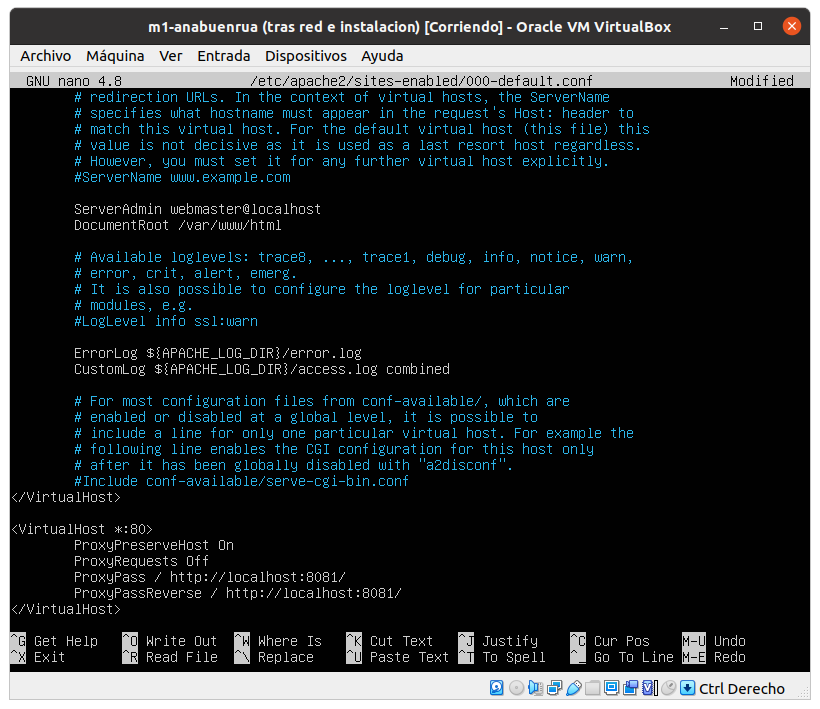
\includegraphics[scale=0.5]{apache_redirect_1}
\end{center}
\end{figure}

Y ejecutamos \verb|sudo a2enmod proxy|, \verb|sudo a2enmod proxy_http|.

Finalmente reiniciamos el servicio: \verb|sudo systemctl restart apache2|.

Finalmente comprobamos que ahora podemos acceder al fichero \verb|swap.html| desde el puerto 8080 en lugar del 8081 que es el por defecto.

\chapter{Curl}

Comprobamos que curl está instalado correcctamente como se ve en \eqref{curl_1}.

\begin{figure}[h!]
\begin{center}
\caption{Comprobando versión de curl}
\label{curl_1}
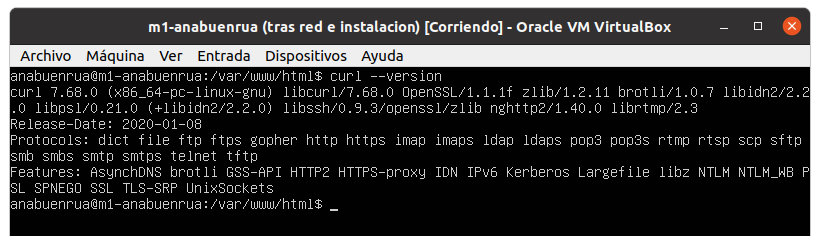
\includegraphics[scale=0.5]{curl_1}
\end{center}
\end{figure}

Accedemos al fichero \verb|swap.html|, creado antes en m1 desde la máquina m2 en \eqref{apache_2}:

\begin{figure}[h!]
\begin{center}
\caption{Accediendo al fichero swap.html de m1 desde m2 }
\label{apache_2}
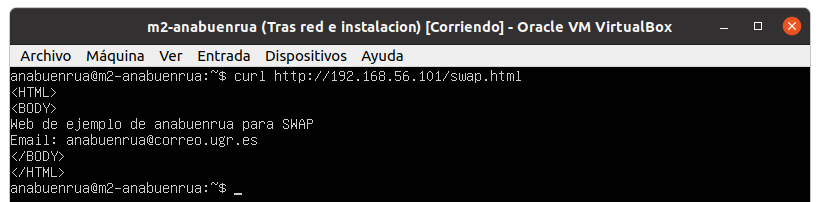
\includegraphics[scale=0.5]{apache_2}
\end{center}
\end{figure}

\section{Opciones -o, -O, -0}

Ahora vamos a usar la opción \verb|-o| o \verb|-output|, que escribe en un fichero la salida de curl en lugar de en la salida estándar.

Por ejemplo, usando de nuevo el fichero \verb|swap.html| escribiendolo en \verb|fichero.html| \eqref{curl_2}

\begin{figure}[h!]
\begin{center}
\caption{Guardando la salida estándar de curl con la opción -o }
\label{curl_2}
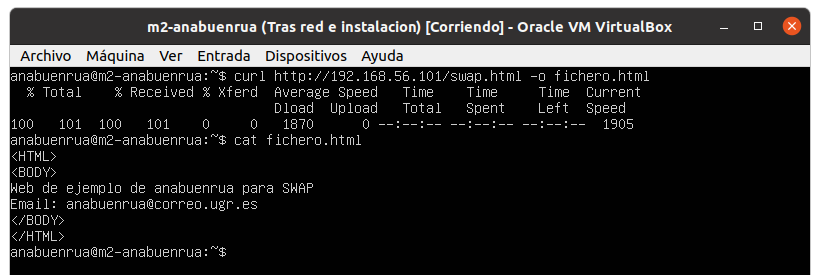
\includegraphics[scale=0.5]{curl_2}
\end{center}
\end{figure}

La opción \verb|-0| sirve para que curl use la versión 1.0 de HTTP en lugar de su versión establecida internamente. Por ejemplo en \eqref{curl_3}

\begin{figure}[h!]
\begin{center}
\caption{Prueba de la opción -0 con curl }
\label{curl_3}
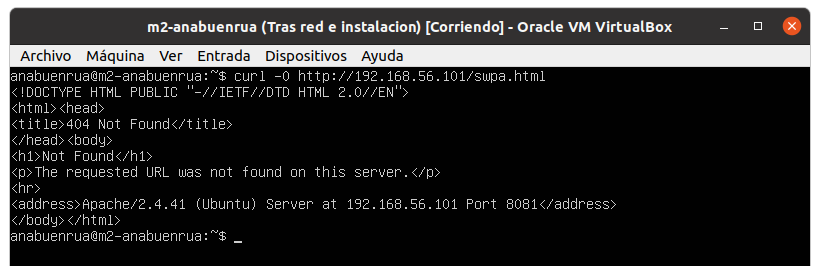
\includegraphics[scale=0.5]{curl_3}
\end{center}
\end{figure}

La opción \verb|-O| guarda el fichero con el nombre con el que está subido, como se ve en \eqref{curl_4}:

\begin{figure}[h!]
\begin{center}
\caption{Prueba de la opción -O con curl}
\label{curl_4}
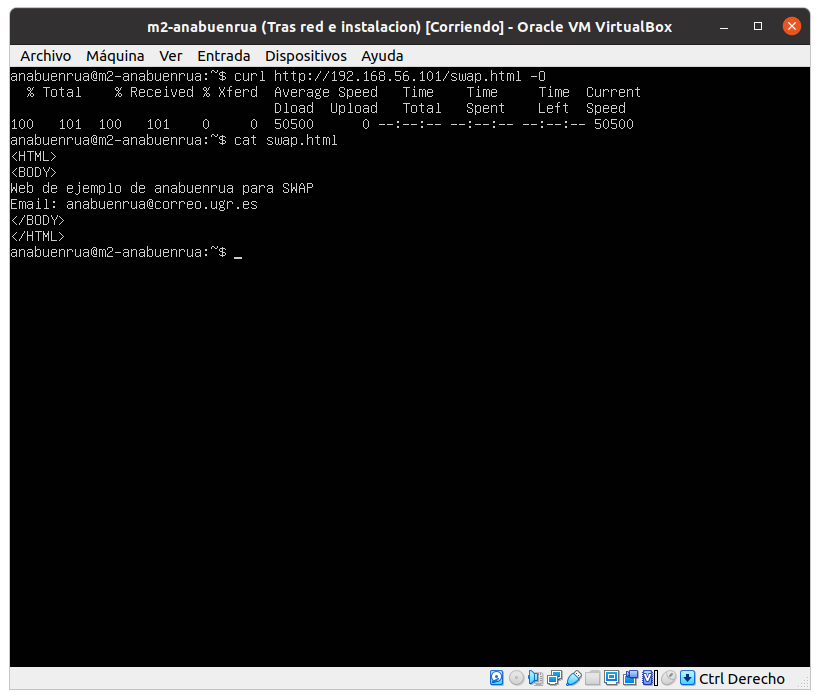
\includegraphics[scale=0.5]{curl_4}
\end{center}
\end{figure}

\section{Peticiones con métodos}

Por defecto, las peticiones que se realizan son usando GET, pero se puede realizar cualquier petición (POST, PUT o DELETE) usando el argumento \verb|--request| o \verb|-X|.

Por ejemplo, realizamos una petición POST adjuntado los datos de \verb|name| y \verb|email| con la opción \verb|-d| como:
\begin{verbatim}
curl -X POST -d 'name=ana&email=anabuenrua@correo' https://example.com/contact.php
\end{verbatim}

Otro ejemplo usando DELETE:
\begin{verbatim}
curl -X "DELETE" https://example.com
\end{verbatim}

\section{Usando cookies}

Con curl podemos manejar cookies mediante las opciones \verb|-c|, para indicar el nombre del archivo donde se guardan las cookies y \verb|-b|, para enviar las cookies.

Comenzamos creando el archivo de las cookies ejecutando:

\begin{verbatim}
curl -c cookies.txt http://www.google.com
\end{verbatim}

Y enseñamos el fichero de cookies \eqref{curl_5}

\begin{figure}[h!]
\begin{center}
\caption{Fichero de cookies cookies.txt}
\label{curl_5}
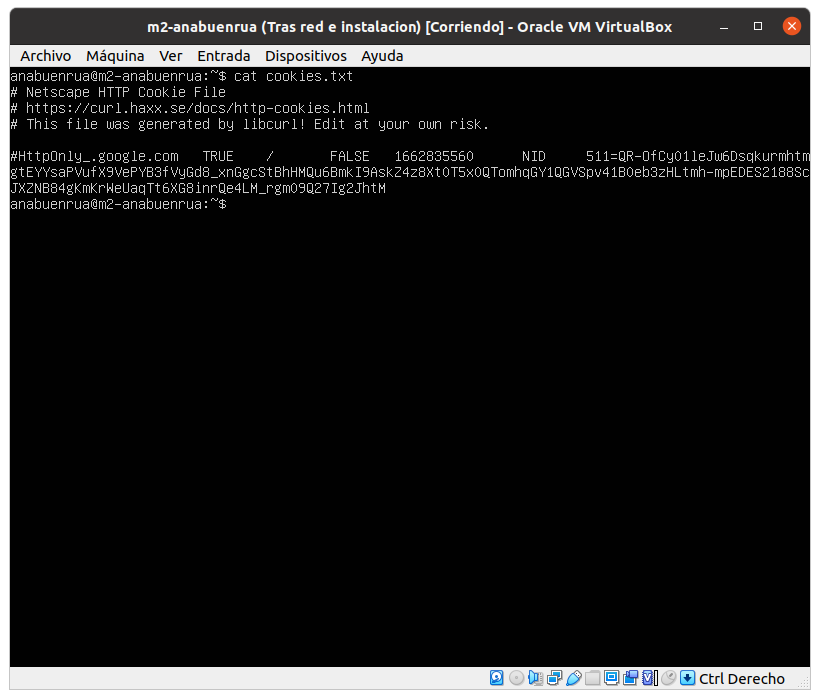
\includegraphics[scale=0.5]{curl_6}
\end{center}
\end{figure}

Y finalmente para enviar las cookies:

\begin{verbatim}
curl -b cookies.txt http://www.google.com
\end{verbatim}

\chapter{SSH}

Para conectarnos entre las máquinas simplemente usamos el comando 

\verb|ssh anabuenrua@<IP maquina>|. Comenzamos conectando de la máquina m1 a m2, y viceversa, como se ve en \eqref{ssh_m1m2} y \eqref{ssh_m2m1}.


\begin{figure}[h!]
\begin{center}
\caption{Conexión por ssh de m1 a m2}
\label{ssh_m1m2}
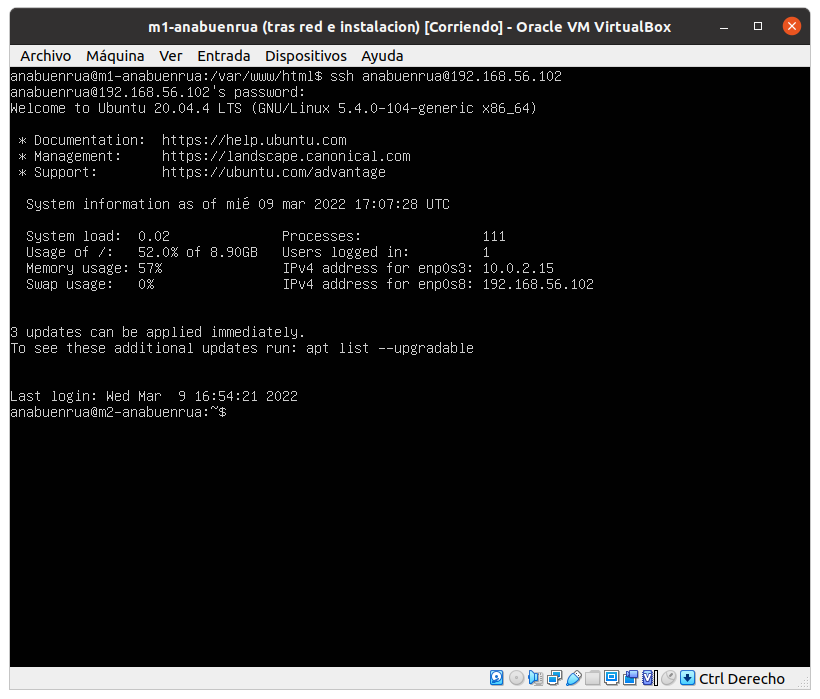
\includegraphics[scale=0.5]{ssh_m1m2_1}
\end{center}
\end{figure}


\begin{figure}[h!]
\begin{center}
\caption{Conexión por ssh de m2 a m1}
\label{ssh_m2m1}
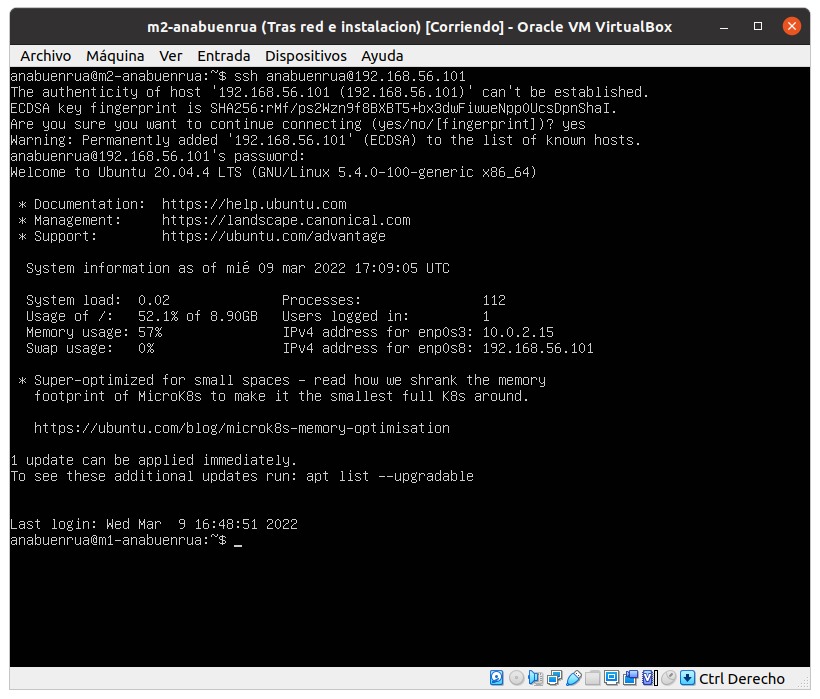
\includegraphics[scale=0.5]{ssh_m2m1_1}
\end{center}
\end{figure}

\section{Cambiando el puerto}

Para cambiar el puerto por defecto que usa ssh cambiamos el fichero \verb|/etc/ssh/sshd_config|, buscamos donde especifica el puerto 22 y lo sustituimos por (por ejemplo) 2022 \eqref{ssh_port_1}:

\begin{figure}[h!]
\begin{center}
\caption{Archivo de configuración /etc/ssh/sshd\_config}
\label{ssh_port_1}
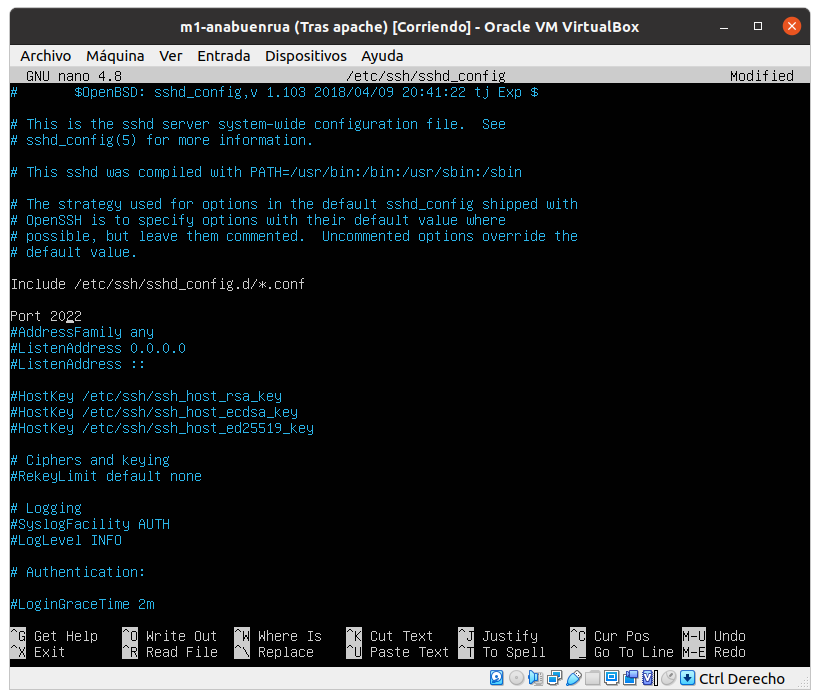
\includegraphics[scale=0.5]{ssh_port_1}
\end{center}
\end{figure}

Y reiniciamos el servicio con \verb|sudo systemctl restart ssh|.

Probamos a conectarnos desde la máquina m2, especificando el puerto con \verb|-p|, si no, no se conecta, como se muestra en \eqref{ssh_port_2}

\begin{figure}[h!]
\begin{center}
\caption{Conexión por ssh al puerto 2022}
\label{ssh_port_2}
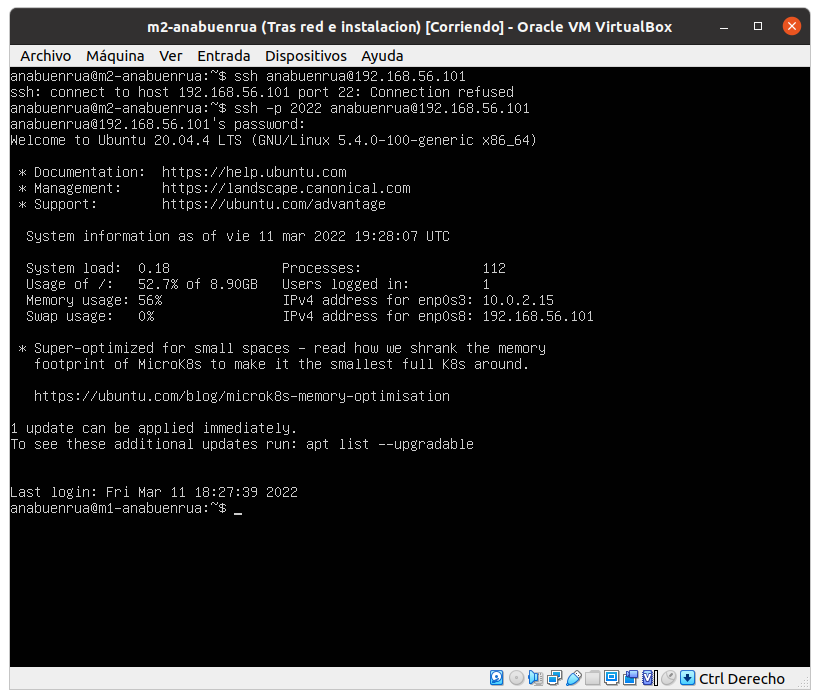
\includegraphics[scale=0.5]{ssh_port_2}
\end{center}
\end{figure}

\section{Acceso sin contraseña}

Finalmente, vamos a configurar el acceso sin contraseña mediante clave pública. Para ello, en cada máquina vamos a generar una clave pública y una clave privada mediante el comando \verb|ssh-keygen|, y dejamos todos los campos por defecto.

Luego copiamos la clave ejecutando en m2: \verb|ssh-copy-id -p 2022 anabuenrua@192.168.56.101| \eqref{ssh_cont_1}.

\begin{figure}[h!]
\begin{center}
\caption{Generación y compartición de clave en ssh}
\label{ssh_cont_1}
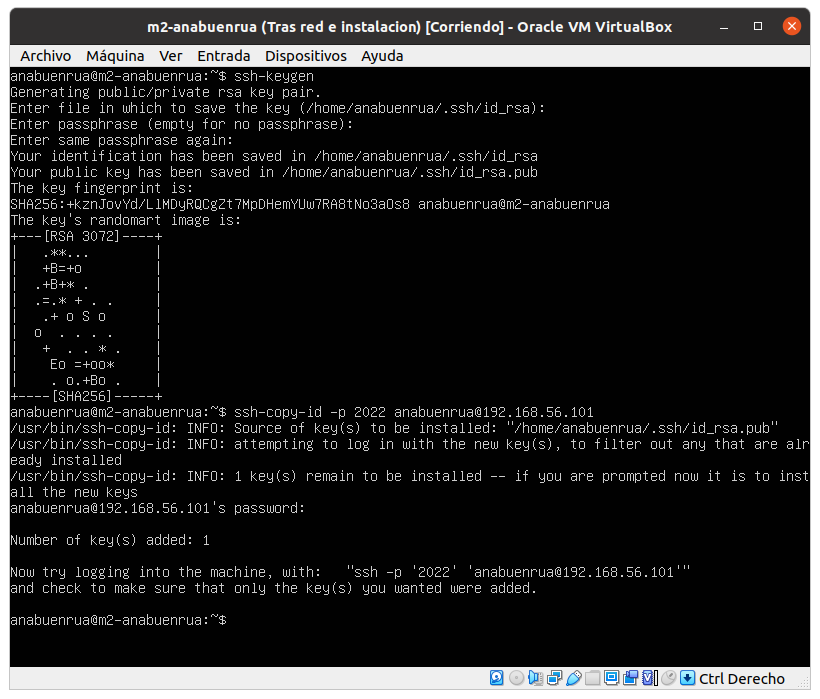
\includegraphics[scale=0.5]{ssh_clave_2}
\end{center}
\end{figure}

Análogamente, en la máquina m1 se ejecuta: \verb|ssh-copy-id anabuenrua@192.168.56.102|.

Tras introducir las contraseñas una sola vez tras la ejecución del comando, ya no será necesario ingresarlas más \eqref{ssh_cont_2}.

\begin{figure}[h!]
\begin{center}
\caption{Conexión por ssh sin contraseña}
\label{ssh_cont_2}
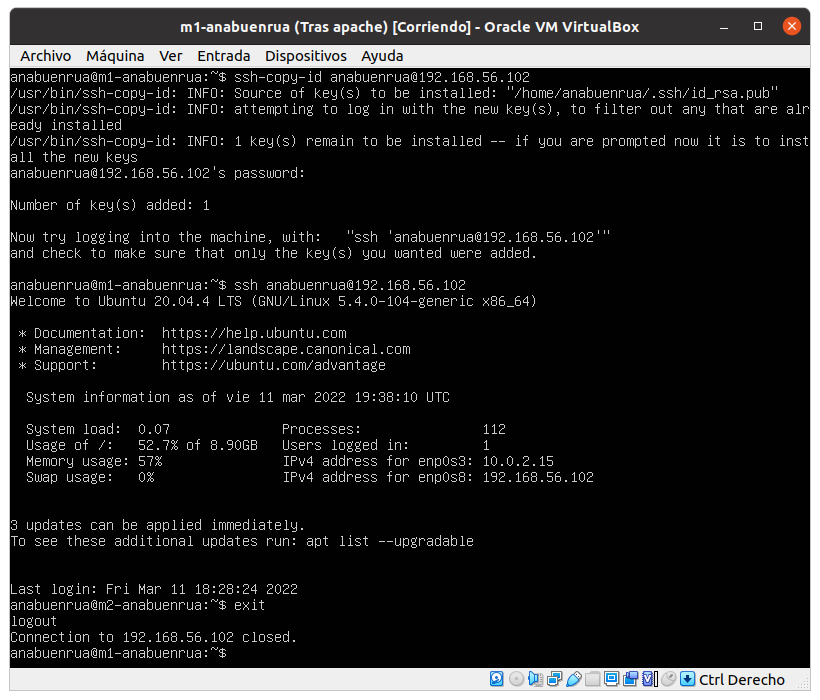
\includegraphics[scale=0.5]{ssh_clave_3}
\end{center}
\end{figure}

